\chapter{Additional Design Diagrams}

\section*{One turn of the diagnostic Copilot}

Figure~\ref{fig:copilot-turn} shows the data flow of one Copilot turn. The server is stateless: the browser carries the case state and sends it with every message.

\begin{figure}[!htbp]
\centering
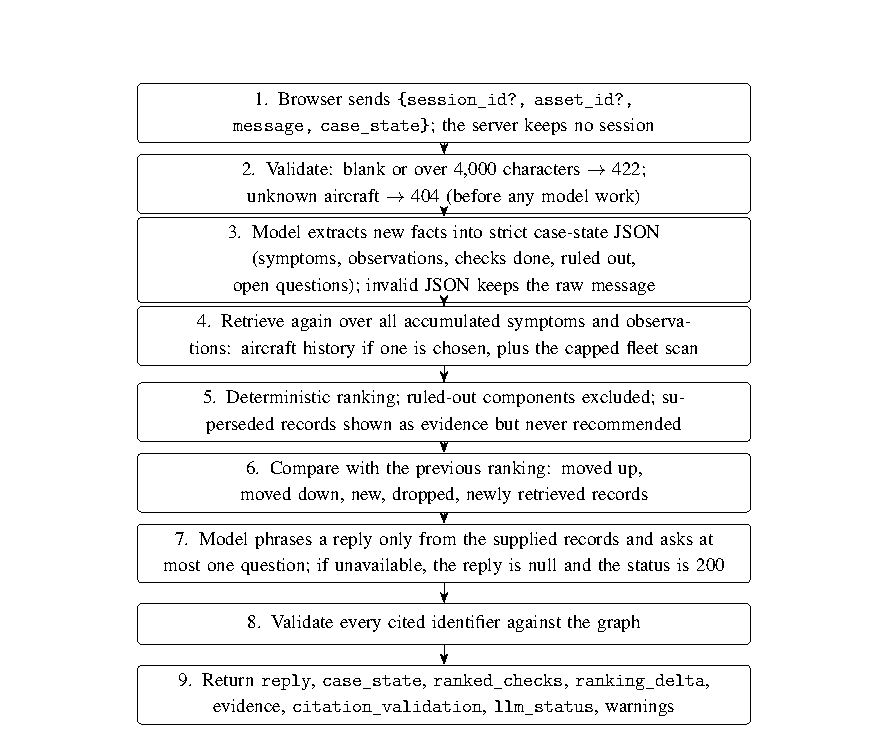
\includegraphics[width=\linewidth,height=0.70\textheight,keepaspectratio]{illustrations/fig_p127_369.pdf}
\caption{Processing of one Copilot turn.}
\label{fig:copilot-turn}
\end{figure}

\section*{Frontend routes and the data they read}

Table~\ref{tab:frontend-routes} maps each frontend route to the page and the principal API endpoints it uses.

\begin{table}[H]
\centering
\caption{Frontend routes and principal endpoints}
\label{tab:frontend-routes}
\small
\begin{tabularx}{\textwidth}{@{}>{\ttfamily\raggedright\arraybackslash}p{0.30\textwidth} >{\raggedright\arraybackslash}p{0.18\textwidth} L@{}}
\toprule
\normalfont Route & Page & Main endpoint(s) \\
\midrule
/app/assets & Assets & \texttt{GET /api/maintenance/assets} \\
/app/asset-history/:id & Asset History & \texttt{GET /api/maintenance/assets/\{id\}/history} \\
/app/records & Service Records & \texttt{GET /api/maintenance/records}, \texttt{/assets} \\
/app/diagnostics & Diagnostics & \texttt{POST /api/maintenance/copilot/turn}, \texttt{/diagnose} \\
/app/review-queue & Review Queue & \texttt{GET /api/review-queue}, \texttt{/corrections}; POST accept/reject \\
/app/maintenance-ingest & Ingest & \texttt{POST /api/maintenance/ingest/upload}, \texttt{/ingest}, \texttt{/records} \\
/app/graph & Knowledge Graph & \texttt{GET /api/graph/overview} \\
/app/settings & Settings / status & \texttt{GET /api/health} \\
\bottomrule
\end{tabularx}
\end{table}
